%\chapter{Machine Learning for Metagenomics and Metatranscriptomics}
%\label{chapter:C}

\section{Abstract}

% ===========================
% ===== INTRODUCTION ========
% ===========================
\section{Introduction}
testing 1, 2, 3.

\subsection{Canonical Correlation Analysis of Metagenomic Gene Expression}



% ================================
% ===== MATERIALS/METHODS ========
% ================================
\section{Materials and Methods}

% =================================
% ===== RESULTS/DISCUSSION ========
% =================================
\section{Results and Discussion}

\subsection{Avoid centering sparse data prior to learning}
\begin{figure}[H]
\centering
    % Originals: /Users/janet/repos/CCA_Omics/code/demo_notebooks/results_for_thesis/170324_example_centered.svg
    % Merged: /Users/janet/Dropbox/thesis/inkscape/170324_standard_scalar.svg.2017_03_24_07_44_42.0.svg
    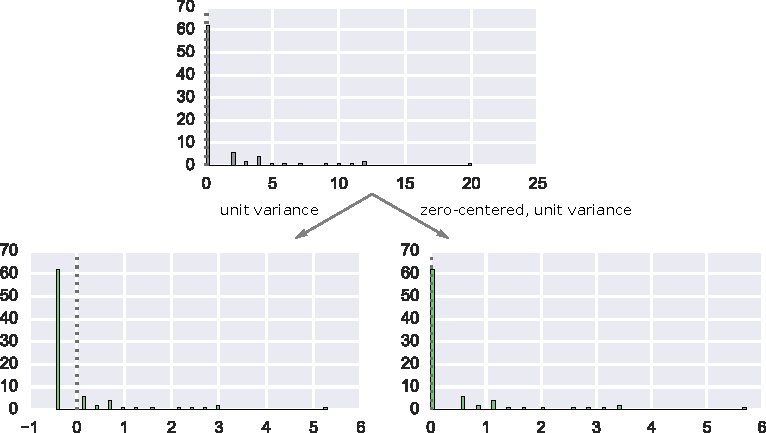
\includegraphics[width=1.0\textwidth]{./tex/chapter3/figures/170324_standard_scalar.pdf}
    \begin{singlespace}
    \caption[Feature scaling: centering sparse features is not advised]{
        When preparing features for machine learning, centering sparse data is not advised.
        The top plot shows the distribution of expression values for a particular copy of a gene encoding
            "methane monooxygenase component A alpha chain".
        The gene is not expressed in many of the samples, giving the large peak at zero.
        Below, two different normalization schemes are shown:
            standardization so the mean is zero and the variance is 1 (left), and
            standardization so the variance is zero (right).
        Machine learning algorithms are likely to use this zero shifted peak as real signal in the model, which is not desired.
        }
    \label{fig:standard_scaler}
    \end{singlespace}
\end{figure}

\begin{figure}[H]
\centering
    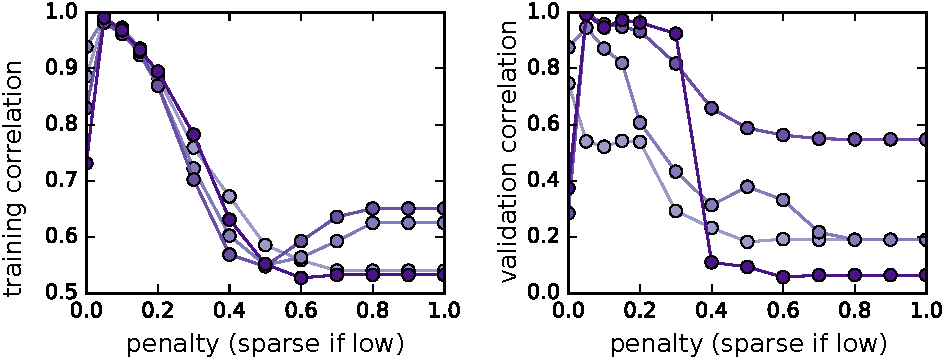
\includegraphics[width=0.9\textwidth]{./tex/chapter3/figures/170324_CCA_not_so_good--cleaned.pdf}
    \begin{singlespace}
    \caption[CCA is not predictive of gene expression for isolate RNA mappings]{
        CCA is not predictive of gene expression for isolate RNA mappings.
        The left two plots are the fit of the model on the training data,
            and the two on the right show how that data predicts on data not included in training.
        Models the left-most point in each series has the strongest regularization (one nonzero coefficient in each vector).
        Each series corresponds to one cross-validation set:
            data was trained on randomly partitioned 3/4 of the data and the corresponding model was used to predict the data in the left-out data.
        }
    \label{fig:cca}
    \end{singlespace}
\end{figure}



% ==========================
% ===== CONCLUSIONS ========
% ==========================
\section{Conclusions}
